\documentclass{beamer}

\usepackage[francais]{babel}
\usepackage[utf8]{inputenc}
\usepackage[T1]{fontenc}
\usepackage{graphicx}
\usepackage{graphics}
\usepackage{color}
\usepackage{textcomp}
\usepackage{pifont}
\usepackage[normalem]{ulem}
\usepackage{times}
\usepackage{hyperref}
\usepackage{verbatim}
\usepackage{amsmath}
\usepackage{amsthm}
\usepackage{amsfonts}
\usepackage[mathscr]{euscript}
\usepackage{pgfpages}
\usepackage{listings}
\usepackage{subfigure}
\usepackage{algorithm}
\usepackage[noend]{algorithmic}
\usepackage{pdftricks}
\usepackage{mathrsfs}
\usepackage{array}
\usepackage{fancybox}
% \usepackage{columns}
\usepackage{multirow}
\usepackage{url}
\usepackage{tikz}
\usepackage{colortbl}
%\usepackage{cite} %DO NOT FUCKING USE CITE ON BEAMER !!! LOST 30 GODDAM' MINUTES ON THIS SHIT !!!
\usepackage{mathabx}
\usepackage{amssymb}
\usepackage{eurosym}
\usepackage{wasysym} % ch0

\let\texteuro\euro

\hypersetup{colorlinks,%
            citecolor=black,%
            filecolor=black,%
            linkcolor=black,%
            urlcolor=blue}

%\addtolength{\parskip}{10pt}

\usetikzlibrary{calc}

\mode<presentation>
\setbeamertemplate{footline}[frame number]
\setbeamercovered{transparent}
\usetheme[navigation]{ESI}

%lst
\definecolor{comment-green}{RGB}{0,166,80}
\lstset{language=C++,
  keywordstyle=\lst@ifdisplaystyle\bf\fi\color{blue!60},
  commentstyle=\color{comment-green},
  stringstyle=\color{red},
  basicstyle=\lst@ifdisplaystyle\tiny\else\tt\fi,
  morekeywords={
    constexpr,concept,decltype,nullptr,nullptr_t,noexcept,final,override},
  frame=single,
  xleftmargin=0.5cm,
  numbers=left,
  tabsize=2}

%title
\subtitle{Langage \texttt{C} / \cpp}
\author{R. Absil}
\date{\today}

%styles
\theoremstyle{definition}
\newtheorem{thm}{Théorème}
\newtheorem{conj}[thm]{Conjecture}
\newtheorem{deff}[thm]{Définition}
\newtheorem{prop}[thm]{Propriété}
\newtheorem{lem}[thm]{Lemme}
\newtheorem*{lem*}{Lemme}
\newtheorem{cor}[thm]{Corollaire}
%\newtheorem{example}{Exemple}
\newtheorem{remark}{Remarque}
\newtheorem{exo}{Exercice}

%typeset
\newcommand{\ie}{{\emph{i.e., }}}
\newcommand{\eg}{{\emph{e.g., }}}
\newcommand{\etal}{{\emph{et al.}}}
\newcommand{\rrceil}{\unichar{"2308}}
\newcommand{\sloand}[2]{\footnote{N. J. A. Sloane - OEIS Foundation - \texttt{www.oeis.org}, Sequence #1 - #2.}}

%math
\newcommand{\IN}{{\mathbb N}}
\newcommand{\IQ}{{\mathbb Q}}
\newcommand{\IR}{{\mathbb R}}
\newcommand{\IZ}{{\mathbb Z}}
\newcommand{\IP}{{\mathbb P}}
\newcommand{\IC}{{\mathbb C}}
\newcommand{\bigo}{{\mathcal{O}}}
\renewcommand{\mod}{\bmod}
\newcommand{\ssi}{\Leftrightarrow}
\newcommand{\then}{\Rightarrow}
\newcommand{\fle}[1]{\stackrel{#1}{\longrightarrow}}
\newcommand{\suchthat}{~\big|~}
\newcommand{\floor}[1]{\left\lfloor #1 \right\rfloor}
\newcommand{\ceil}[1]{\left\lceil #1 \right\rceil}
\DeclareMathOperator*{\argmin}{argmin}
\DeclareMathOperator*{\argmax}{argmax}

%tikz
\tikzstyle{_vertex}=[fill=white, circle,minimum size=12pt,inner sep=1pt]
\tikzstyle{_blackv}=[fill=black, circle,minimum size=8pt,inner sep=1pt]
\tikzstyle{_dot}=[fill=black, circle, minimum size = 1mm, inner sep=0pt]
\tikzstyle{_bigvertex}=[fill=white, circle,minimum size=21pt,inner sep=1pt]
\tikzstyle{_arc}=[->, >=stealth]
\tikzstyle{_boldarc}=[->, >=stealth, line width=2pt]

\newcommand{\cpp}{\texttt{C++}}
\newcommand{\java}{\texttt{Java}}


\title{Ch. 0 - Présentation}

\begin{document}
\begin{frame}
  \titlepage
\end{frame}

\begin{frame}
  \frametitle{Table des matières}
  \footnotesize \tableofcontents[pausesections,pausesubsections]
\end{frame}


\section{Introduction} 

\begin{frame}
\frametitle{Le prof}
\begin{itemize}[<+->]
\item Vous m'avez peut-être connu en math et comptabilité
\item Derrière le «~fasciste~» se cache un prof plus modéré \smiley
	\begin{itemize}
	\item Vous n'êtes plus des 1\textsuperscript{ères}
	\item Vous êtes «~grands~»
	\end{itemize} 
\item Si vous avez une question, posez-là
	\begin{itemize}
	\item Je ne mords pas
		\begin{itemize}
		\item ... trop
		\item ... souvent
		\end{itemize}
	\end{itemize}
\item Le \cpp\ est un langage plus technique que le \java
	\begin{itemize}
	\item Si vous ne comprenez pas, j'ai peut-être tout simplement mal expliqué
	\end{itemize}
\end{itemize}
\end{frame}

\section{Le cours}

\begin{frame}
\frametitle{Fréquence}
\begin{itemize}[<+->]
\item Cours donné $6$h par semaine
\item 4h de théorie, 2h de labo
	\begin{itemize}
	\item Déséquilibre «~historique~» post-décret
	\end{itemize}
\item Présence «~facultative~»
	\begin{itemize}
	\item ... mais vous prenez vos responsabilités
	\end{itemize}
\item Le support de théorie est conçu \emph{pour moi}
	\begin{itemize}
	\item Vous êtes vivement encouragés à prendre des notes
	\end{itemize}
\end{itemize}
\end{frame}

\begin{frame}
\frametitle{Pourquoi un cours de \texttt{C} / \cpp}
\begin{itemize}[<+->]
\item Bien que disposant de parts de marchés discutables, ces langages restent très présents
	\begin{itemize}
	\item Systèmes d'exploitation
	\item Micro-embarqué
	\item Jeux vidéo
	\item Sécurité
	\end{itemize}
\item Important d'être capable de pouvoir se prétendre développeur \texttt{C} / \cpp
\item Pouvoir maintenir d'anciens programmes et en concevoir de nouveaux
\end{itemize}
\end{frame}

\begin{frame}
\frametitle{Objectifs du cours de \texttt{C} / \cpp}
\begin{itemize}[<+->]
\item Acquérir une bonne maîtrise des concepts liés à ces deux langages
\item Pouvoir se démarquer de ses habitudes de programmations liées à d'autres langages
	\begin{itemize}
	\item Même si les syntaxes sont similaires, \cpp\ et \java\ sont \emph{très} différents
	\item Les bons réflexes \java\ sont souvent de mauvais idiomes \cpp
	\end{itemize}
\item Acquérir de bonnes pratiques de programmations
	\begin{itemize}
	\item Certains affirment que le langage est sournois
	\item Ce n'est pas le cas \emph{si} on suit de bonnes pratiques
	\item Cela implique de se discipliner
	\end{itemize}
\end{itemize}
\end{frame}

\begin{frame}
\frametitle{Le support}
\begin{itemize}[<+->]
\item Transparents disponibles en deux versions
	\begin{enumerate}
	\item \texttt{slides.pdf} : version avec pauses
	\item \texttt{slides-handout.pdf} : version imprimable
	\end{enumerate}
\item Les slides contiennent des \emph{extraits} de code
	\begin{itemize}
	\item Les codes complets sont référencés, et disponibles dans le répertoire \texttt{codes}
	\item On travaillera systématiquement avec les codes complets, à compiler et commenter
	\end{itemize}
\item L'intégralité des supports est disponible sur \url{https://gitlab.com/rabsil/c-cpp}
	\begin{itemize}
	\item Repository public
	\end{itemize}
\end{itemize}
\end{frame}

\section{Évaluation}

\begin{frame}
\frametitle{Modalités}
\begin{itemize}[<+->]
\item UE intégrée
	\begin{itemize}
	\item Les bonnes notes d'une AA «~compensent~» les mauvaises de l'autre
	\end{itemize}
\item Note finale : ??\% théorie, ??\% laboratoires
\item Deux interrogations «~bonus~» de théorie
	\begin{itemize}
	\item La note compte si leur résultat est plus important que l'examen
	\end{itemize}
\item Une interrogation non bonus de laboratoire (??\%)
\item Examen oral de théorie
	\begin{itemize}
	\item 10 minutes de préparations, 30 minutes d'exposé
	\end{itemize}
\item Examen (machine) de laboratoire
\item Modélités complètes et détaillée sur PoÉSI
\end{itemize}
\end{frame}

\begin{frame}
\frametitle{Questions}
\begin{center}
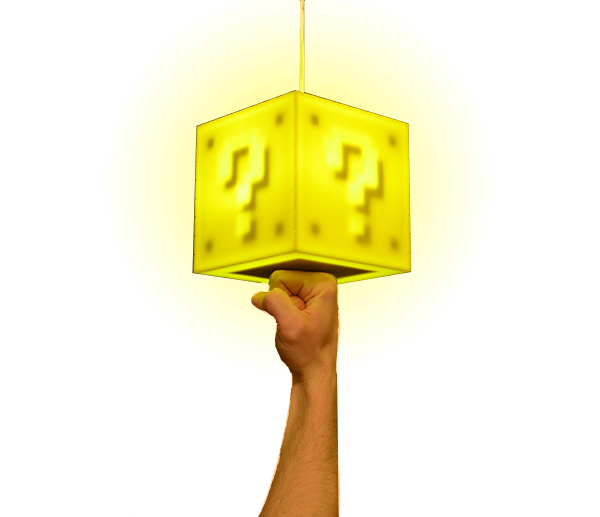
\includegraphics[height=6cm]{pics/question-3.png}
\end{center}
\end{frame}

\end{document}
